\subsection{Quelle protections sont mises en place contre les attaques par fautes ?}

Bien que l'algorithme de l'AES est incassable aujourd'hui, son implementation peut permettre de récupérer des données sensibles par de nombreux moyens.
Dans ce TP, on s'intéresse à une potentielle attaque par injection de fautes et a une contre-mesure de cette attaque. 
Pour mener un attaque par faute  dans ce module AES, nous avons tout d'abord analysé le circuit et tenté de comprendre comment le système était protégé.\\

La sécurité du chiffrement tel qu'il est implémenté pour ce TP réside dans la redondance d'information. 
En effet, chaque calcul sur les octets du data_unit sont fait 2 fois, cela permet, à l'issue des deux calculs, de comparer que les 2 résultats sont identiques. 
Dans ce cas, aucune faute ne sera détectée. En revanche, si l'un des deux calculs ne donne pas le même résultat, un flag sera levé, et le calcul sera considéré comme erroné.\\

De plus, il est possible de doubler le nombre de calculs effectué par round, sans pour autant doubler le temps de calculs. 
En effet, d'après la figure~/ref{fig:DDR} page~/pageref{fig:DDR} montre que durant les 6 premiers cycles 12 calculs sont effectués (sur fronts montant et descendant) 
et sur les 6 cycles suivants, les mêmes calculs sont à nouveau effectués. 
Ainsi si l'assaillant change une donnée du circuit, le calcul fait sur les 6 premiers cycles et celui fait sur les 6 derniers seront surement différents et une erreur sera levée.

\begin{figure}
\begin{figure}[htbp]
\begin{center}
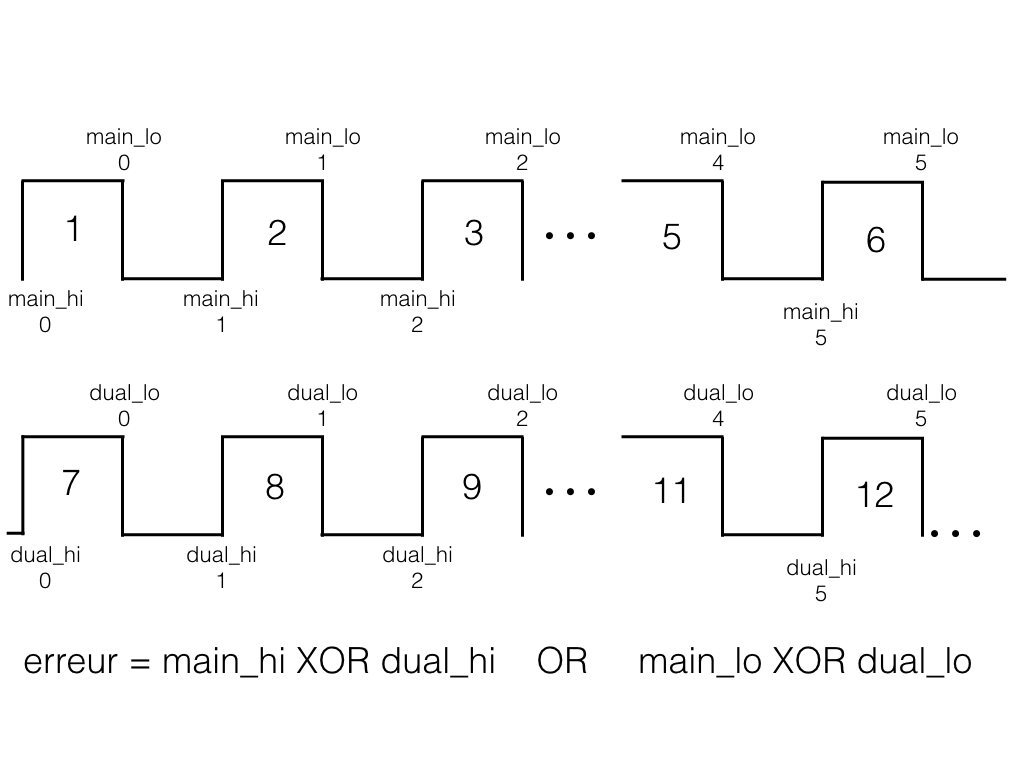
\includegraphics[scale=1.0]{DDR}
\caption{Exemple de Double Data Rate}
\label{fig:DDR}
\end{center}
\end{figure}

\subsection{Quelles sont les faiblesses de cette sécurité ?}

Le problème avec cette façon de sécurisé l'AES est que si l'on change la valeur d'un octet pendant exactement 6 cycles, la valeur du premier calculs sera identique au deuxième calcul. 
Ainsi, il ne sera plus possible de faire remonter l'erreur. Cela permettrai à l'attaquant de faire changer un octet d'un 

\subsection{Implémentation de l'attaque par faute}

\subsection{Embarcation du code}
